\documentclass[a4paper]{article}
\usepackage[brazil]{babel}
\usepackage[T1]{fontenc}
\usepackage{graphicx}
\usepackage{listings} 
\usepackage{amsfonts}
\usepackage{mathabx}
%%%%%%%%%%%%%%%%%%%%%%%%%%%%%%%%%%%%%%%%%
% Arsclassica Article
% Structure Specification File
%
% This file has been downloaded from:
% http://www.LaTeXTemplates.com
%
% Original author:
% Lorenzo Pantieri (http://www.lorenzopantieri.net) with extensive modifications by:
% Vel (vel@latextemplates.com)
%
% License:
% CC BY-NC-SA 3.0 (http://creativecommons.org/licenses/by-nc-sa/3.0/)
%
%%%%%%%%%%%%%%%%%%%%%%%%%%%%%%%%%%%%%%%%%

%----------------------------------------------------------------------------------------
%	REQUIRED PACKAGES
%----------------------------------------------------------------------------------------

\usepackage[
nochapters, % Turn off chapters since this is an article        
beramono, % Use the Bera Mono font for monospaced text (\texttt)
eulermath,% Use the Euler font for mathematics
pdfspacing, % Makes use of pdftex’ letter spacing capabilities via the microtype package
dottedtoc % Dotted lines leading to the page numbers in the table of contents
]{classicthesis} % The layout is based on the Classic Thesis style

\usepackage{arsclassica} % Modifies the Classic Thesis package

\usepackage[T1]{fontenc} % Use 8-bit encoding that has 256 glyphs

\usepackage[utf8]{inputenc} % Required for including letters with accents

\usepackage{graphicx} % Required for including images
\graphicspath{{Figures/}} % Set the default folder for images

\usepackage{enumitem} % Required for manipulating the whitespace between and within lists

\usepackage{lipsum} % Used for inserting dummy 'Lorem ipsum' text into the template

\usepackage{subfig} % Required for creating figures with multiple parts (subfigures)

\usepackage{amsmath,amssymb,amsthm} % For including math equations, theorems, symbols, etc

\usepackage{varioref} % More descriptive referencing

%----------------------------------------------------------------------------------------
%	THEOREM STYLES
%---------------------------------------------------------------------------------------

\theoremstyle{definition} % Define theorem styles here based on the definition style (used for definitions and examples)
\newtheorem{definition}{Definition}

\theoremstyle{plain} % Define theorem styles here based on the plain style (used for theorems, lemmas, propositions)
\newtheorem{theorem}{Theorem}

\theoremstyle{remark} % Define theorem styles here based on the remark style (used for remarks and notes)

%----------------------------------------------------------------------------------------
%	HYPERLINKS
%---------------------------------------------------------------------------------------

\hypersetup{
%draft, % Uncomment to remove all links (useful for printing in black and white)
colorlinks=true, breaklinks=true, bookmarks=true,bookmarksnumbered,
urlcolor=webbrown, linkcolor=RoyalBlue, citecolor=webgreen, % Link colors
pdftitle={}, % PDF title
pdfauthor={\textcopyright}, % PDF Author
pdfsubject={}, % PDF Subject
pdfkeywords={}, % PDF Keywords
pdfcreator={pdfLaTeX}, % PDF Creator
pdfproducer={LaTeX with hyperref and ClassicThesis} % PDF producer
} 
\hyphenation{Fortran hy-phen-ation}

\title{\normalfont\spacedallcaps{Projeto Interativo III  Angry Robots}}

\author{Carolina Bomfim, Mahaira Soares de Souza, \\ Rafael da Silva Santos e Thiago Messias } 
 

\date{} 



\begin{document}




\pagestyle{scrheadings} 


\maketitle

{\large caroline.bomfim@hotmail.com.br, mahaira\_souza@hotmail.com, rafa\_silva.santos@hotmail.com, messiasthi@gmail.com}
\\
\\
\\
\\

\hspace{0.45\textwidth} 
   \begin{minipage}{.5\textwidth}
   \large "Angry Robots, é um jogo baseado em visão computacional, desenvolvido em linguagem C, versão 99, ultilizando a biblioteca allegro 5, que possibilitou criar a interface gráfica do jogo. A principal interação do mesmo é através de uma câmera, ultilizando a biblioteca OpenCV para desenvolver estes aspectos. Apresentado para a conlcusão da disciplina, Projeto Interativo III, do bacharelado em Ciência da Computação, Centro Universitário Senac."\\[0.1cm]
			Sob orientação do Prof.º: Marcelo Hashimoto.
  \end{minipage}
  \vfill

\vspace{1cm}


\section*{Resumo}

Angry Robots, jogo originalmente criado por jovens do 
3º semestre de Ciência da Computação, desenvolvido no decorrer do semestre
proposto na disciplina de Projeto Interativo, com bibliotecas como
OpenCV - "biblioteca totalmente multiplataforma, livre para o
ambito acadêmico e comercial também, utilizado para desenvolver
aplicações em visão computacional", allegro - "biblioteca gráfica
de código aberto com principal objetivo de games 2D". Atualmente
existem muitos jogos no mercado cuja a interação é através de
câmeras, desde jogos de dança, até jogos de aventura, neste
programa em específico os algoritmos essênciais foram calculo de
mediana, conversão para escala de cinza, segmentação e corte e
centroide.\\
\\
{\bf Palavras-chave:} algoritimo, OpenCV, allegro, biblioteca gráfica.
\\


\section*{Abstract}

{\it Angry Robots, game originally created by young people from the 3rd semester of Computer Science, developed during the semester proposed in discipline Interactive Project with libraries like OpenCV - "totally multiplatform library, free for academic and business scope also used to develop applications in computer vision ", allegro -" open source graphics library with main objective of 2D games. Nowadays there are a lot of games that the main interaction is through of cameras, there are games about dance, adventure and so on. In this program the main algorithms was calculate median, converting to garyscale, cutting and threading, and many others."\\

{\bf Keywords:} algorithm, OpenCV, allegro, graphics library.} 
\\


\section*{Introdução}

Segundo pequisas[4], jogos que necessitam de movimentos rápidos e
de raciocinio lógico por meio da interatividade das câmeras ajudam
desenvolver a coordenação motora, agilidade, criatividade,
percepção corporal e o equilíbrio físico e mental (Chamado de ponto
de equilibrio entre o cerebro e o corpo), a grande chave de tudo é
que isso acontece de uma forma divertida, e muitas vezes o jogador
nem percebe que desenvolveu estas habilidades. Angry Robots foi
feito pensando nestes aspectos, pois o mesmo faz com que o usuário
se movimente para poder atingir ou desviar de objetos e concluir
com sucesso o objetivo do jogo.
\\
\section*{Revisão de Literatura}

Não houve um jogo especifico em que nos baseamos, queríamos
algo diferente pouco utilizado, em questão do OpenCV e allegro juntos.
Em busca de um jogo futurista, começamos pelo ambiente onde se
passaria o enredo do mesmo, e para a nossa sorte a primeira imagem
que apareceu era de um Cyborg, claro, a partir daquele instate
sabíamos que a história teria um robô, como personagem principal. A
segunda parte de escolhas foi adaptar a nossa ideia a realidade
atual, precisávamos ambientar algo futurista em 2D, já que o
allegro não nos permite ir muito além. Pesquisamos diversos jogos
com robôs e um site em especifico nos chamou atenção: Laboratório
Garagem *LINK*, porém todos fugiam do ambiente proposto para nós, a
maioria dos mesmo utilizavam arduinos, OpenCV e python, enquanto
deveríamos desenvolver em Allegro 5, Linguagem C e OpenCV, a grande
dificuldade foi o código de rastremento já que não havia base.
\\
\section*{Desenvolvimento}
\begin{enumerate}

\item{RGB}\\

A conversão para escala de cinza é feita usando o sistema de cores RGB[5], (Red, Blue, Green). \\

\begin{figure}[!htb]
\centering

\includegraphics{peq.png}
\caption{representação rgb}
\label{Rotulo}
\end{figure}


Isso possibilita a ultilização de todas as outras apenas usando azul, verde e vermelho, assim como o exemplo abaixo:\\

ALLEGRO\_COLOR blue = al\_map\_rgb(0,0,255); \\
ALLEGRO\_COLOR green = al\_map\_rgb(0,255,0); \\
ALLEGRO\_COLOR red = al\_map\_rgb(255,0,0); \\
\\
Este método permite um melhor rastreamento, mais rápido por não se tratar de 3 váriaveis sendo usadas
simultaneamente mas apenas com uma, onde seus valores váriavam de 0 a 255. O valor 255 é o limite que a variavel atinge
por se tratar de uma única escala com base na captação de luz por uma camera, onde cada bit tem valor maximo de 2\^8.\\
Essa limitação transforma as opções de tratamento em algo limitado, facilitando o número de algoritmos que podem ser
usardos \\
\\
\item{Mediana}


A mediana[6] (m=fi/2) mostra o número central de um grupo, ou seja, os números são ordenados e o elemento que estiver no meio é a mediana, esse método é ultilizado para tornar mais definido o degradê da luz, definindo assim uma borda onde as funções feitas para usar essa borda para fazer os próximos calculos necessários para o programa obter a posição do objeto. Observe o exemplo abaixo: \\


\begin{lstlisting}
int aux = 0;
 unsigned char buffer[9];
 for(int dy = -1; dy < 1; dy++){
  for(int dx = -1; dx < 1; dx++, aux++){
   buffer[aux] = imagem[y+dy][x+dx];
  }
 }
 for(aux = 0; aux < 8; aux++){
  for(int l = 0; l < aux; l++){
   if(buffer[l] > buffer[l+1]){
    int n = buffer[l];
    buffer[l] = buffer[l+1];
    buffer[l+1] = n;
   }
  }
 }
 imagem[y][x] = buffer[4];
}
else{
 return;
}
\end{lstlisting}

\item{Limiar}
\\

O valor limiar define um limite mínimo de uma duração. Se uma duração ultrapassar do limite especificado o valor limiar será utilizado.
No jogo, o valor limiar e utilizado para o efeito de luz sobre o corpo, se o efeito da luz do ambiente passar do limite minimo para a camera reconhecer o movimento ou objeto, o valor limiar irá ignorar a luz vindo do ponto especifico do ambiente para que não atrapalhe no reconhecimento do movimento do jogo.
Esse tratamento é conhecido como histograma, onde todos os valores são dispostos em um gráfico e todos os valores que superam a marca minima são elevados ao valor máximo do histograma e os que não chegam a marca são rebaixados ao valor minimo do gráfico. 
\\
Veja no exemplo abaixo:

\begin{figure}
\centering
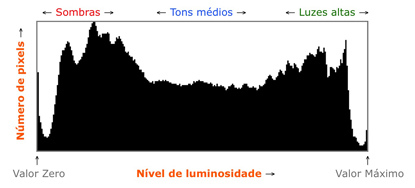
\includegraphics{histograma2.jpg}
\caption{Exemplo de histograma}
\end{figure}

\item{Segmentação e Corte}
\\
O algoritmo de segmentação e corte foi utilizado para que se possa diminuir a zona de rastreamento do jogo, segundo pesquisas, os usuários não utilizam os cantos superios e inferiores quando jogam, procuram se focar no centro da tela e consequentemente no centro da camera, dessa forma tendo uma melhor visão do jogo. Sabendo disso as partes exteriores da tela foram ignorar, almentando a velocidade do algoritmo e aprimorando o a zona rastreada.

Veja o algoritmo que faz a segmentação e o corte:

\begin{lstlisting}
int larg = largura/8;
int alt = altura/8;
int count = 1, count1 = 1;
while(count1 <= 8){
int x0 = 0; 
int x1 = larg;
while(count <= 8){
  int y0 = 0;
  int y1 = alt;
  if(x0 != 0 && y0 != 0){
    histograma(imagem, x0, x1, y0, y1);
  }
  y0 += y1;
  y1 += alt;
  count++;
}
x0 += x1;
x1 += larg;
count1++;
}
\end{lstlisting}
\end{enumerate}
\section*{Resultados}
Na produção desse jogo foi utilizado conhecimentos amplamente desenvolvios no 2ºSemestre do curso com a biblioteca Allegro, o desenvolvimento principal trabalhado nesse projeto foi o da biblioteca OpenCV utilizando as funções limitadas pelo orientador o desenvolvimento foi em sua maior parte focado em algoritmos de alto desempenho focando a precisão e a variação de luminosidade, trabalhando de uma forma que o ajuste seja fácil.
\begin{figure}[!htb]
\centering
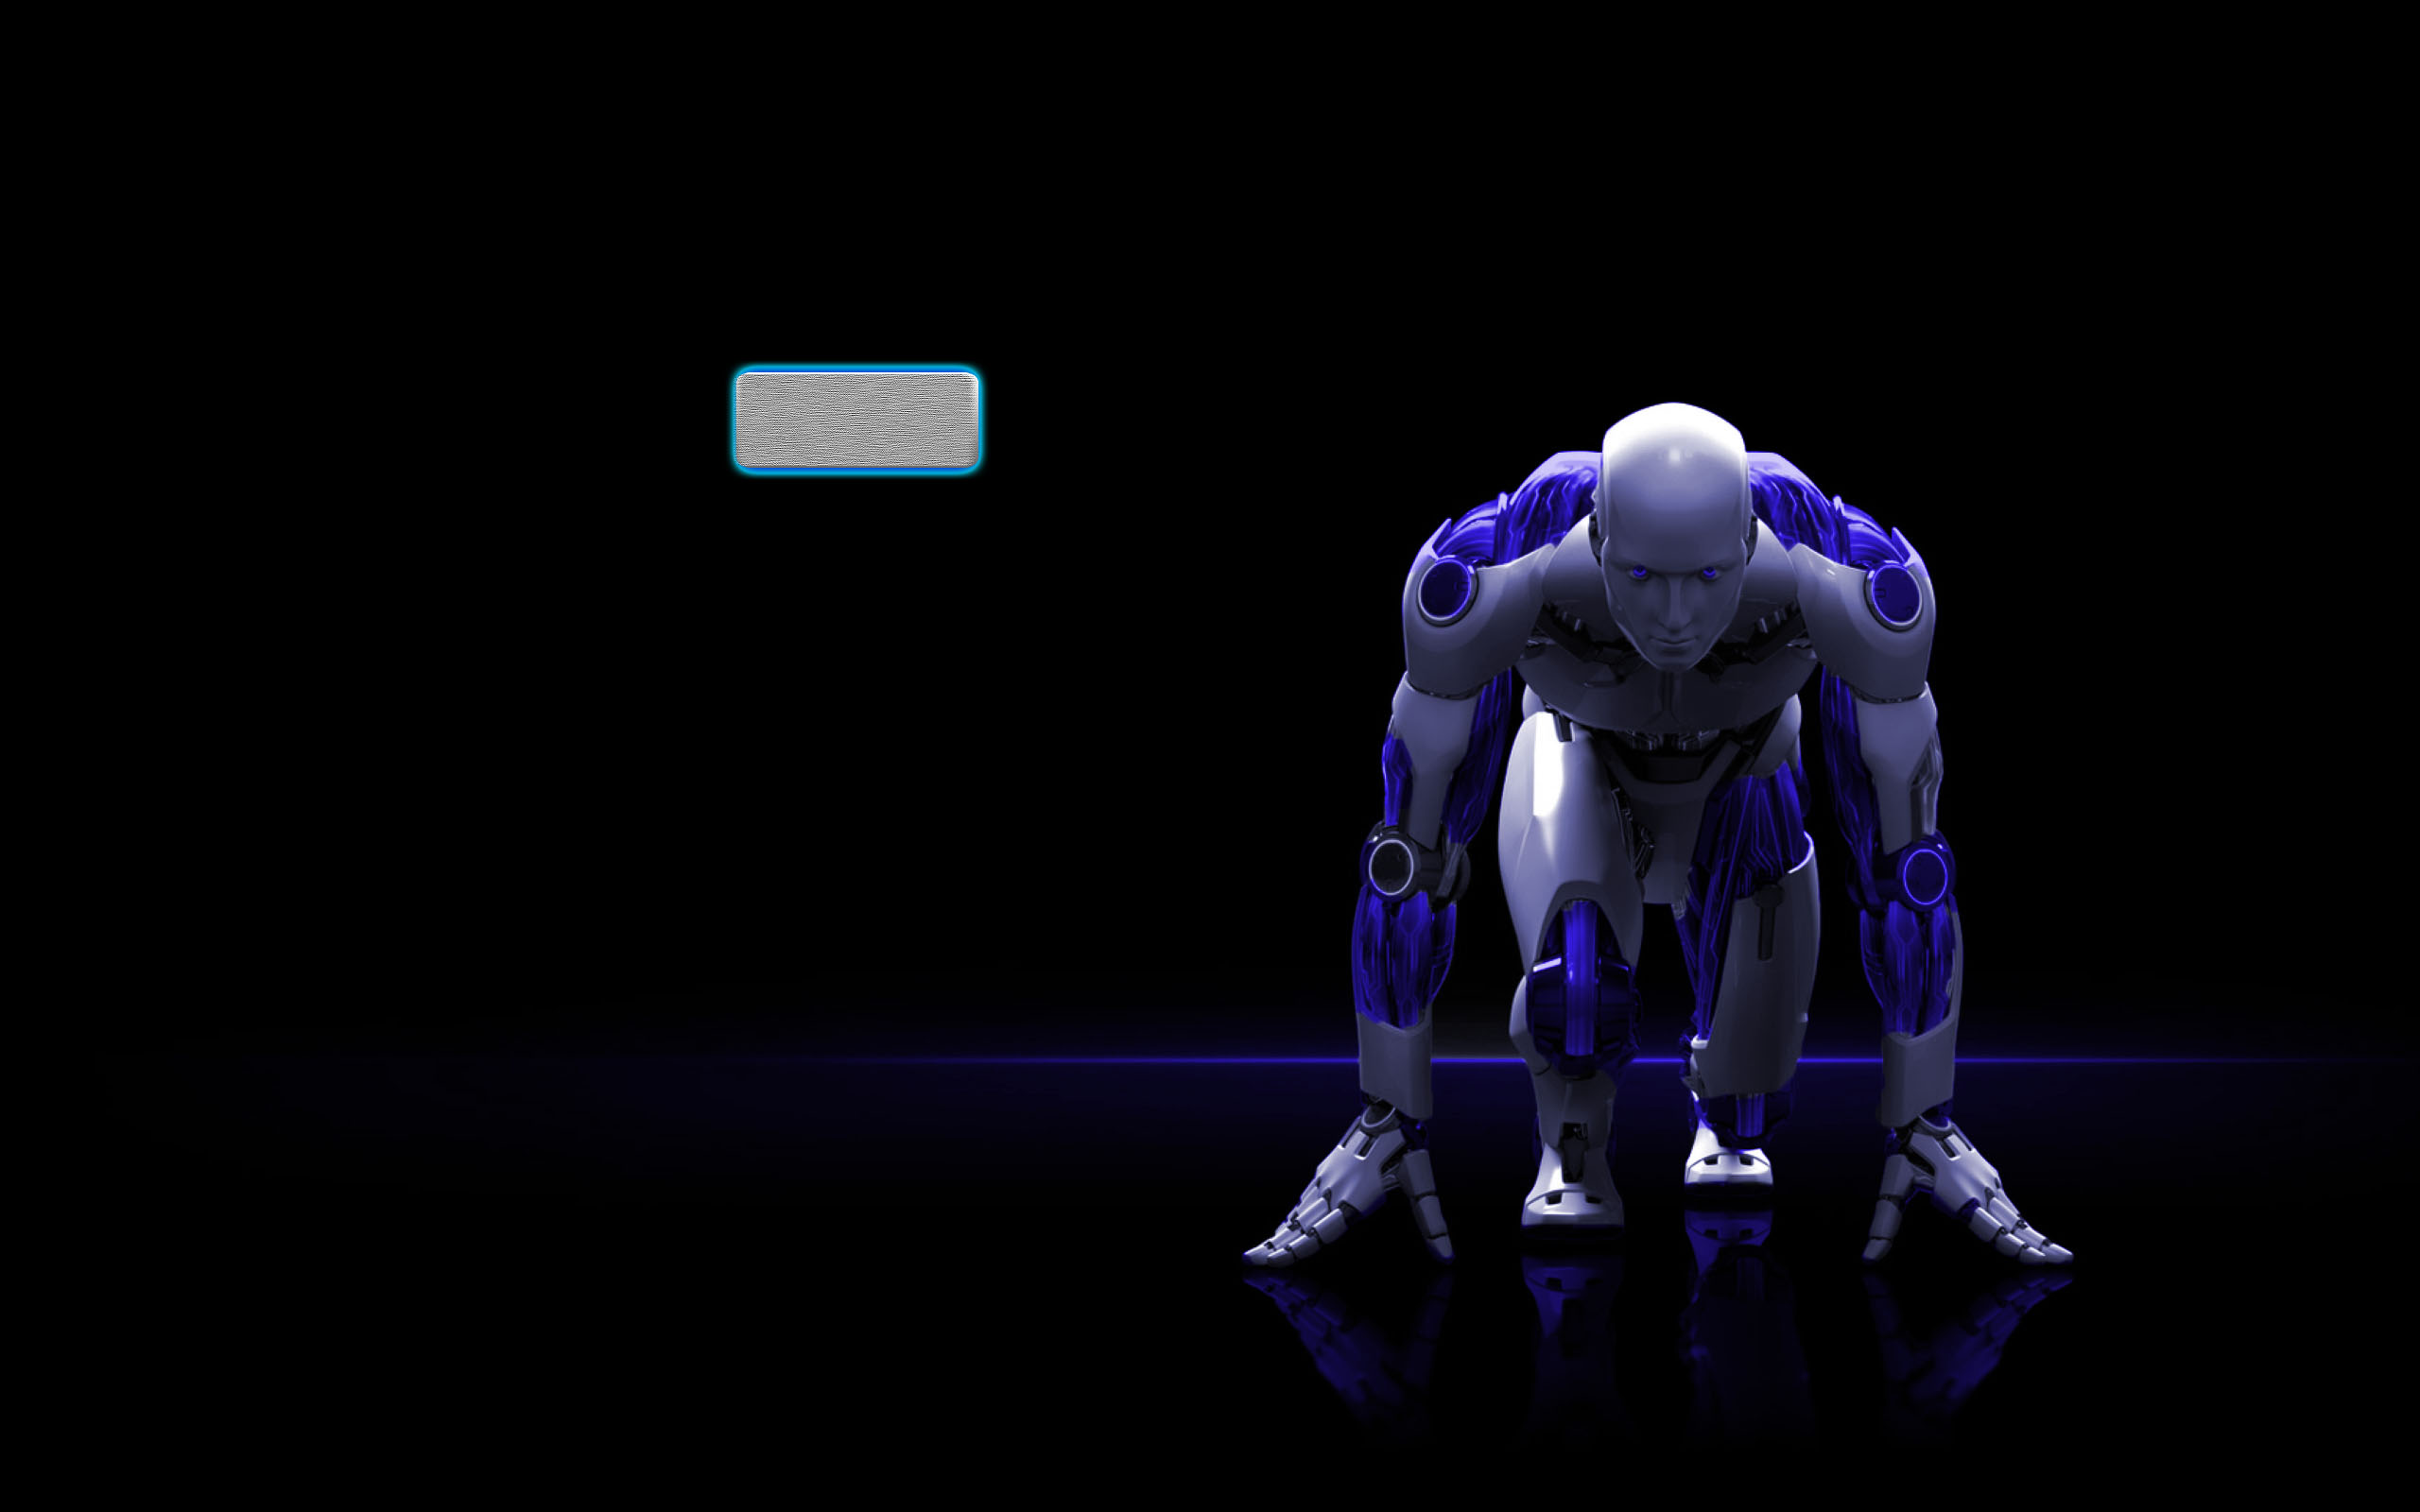
\includegraphics{robot.jpg}
\caption{representação rgb}
\label{Rotulo}
\end{figure}
\section*{Considerações Finais}
Neste programa, o rastreamento pode ser considerado uma das partes mais demoradas e difíceis de desenvolver, pois alguns fatores atrapalharam, o principal deles foi a iluminação, dependendo do local o jogo não conseguia fazer o rastreamento correto, porém isso foi corrigido mais tarde usando calculo de mediana e histograma ajustando-os de acordo com a iluminação. Foi constatado também que a conversão da imagem para uma única escala 256 melhora o processamento necessário e o gasto da memória. Em um programa que envolve um alto número de interações em um curto periodo de tempo é uma constatação essencial.
O projeto proporcionou uma maior habilidade em lógica, linguagem C, calculos com baixo custo computaional resultando em  visão computacional, pois todos esses itens foram fundamentais para o desenvolvimento do jogo.

\begin{thebibliography}{7}
\bibitem{Linguagem C} Como Programar em C \\
\newblock H.M. Deitel P.J. Deitel

\bibitem{Allegro 5} http://www.rafaeltoledo.net/tutoriais-allegro-5/ \\
\newblock Allegro 5

\bibitem{OpenCv} http://opencv.org/ \\
\newblock OpenCV

\bibitem{R7}http://noticias.r7.com/tecnologia-e-ciencia/noticias/jovens-apelam-para-games-corporais-para-melhorar-condicionamento-fisico-20110527.html
\\
\newblock Portal R7 de notícias

\bibitem{RGB} http://www.significados.com.br/rgb/
\\
\newblock RGB

\bibitem{Mediana}http://educacao.uol.com.br/matematica/estatistica-moda-mediana.jhtm
\\
\newblock Calculo de mediana

\bibitem{ Centróide} http://www.ipb.pt/~lmesquita/nova/04-05/mec/cap6.PDF
\\
\newblock Centróide 
\end{thebibliography}
\end{document}